\chapter{Phase 3: Fein-Design und Installation/Konfiguration}
Text Phase 3 kommt hier...

\section{Package Diagram}
Das Smartwatch besitzt einige interessante Funktionen: einen präzisen Touchscreen, Apps und Widgets, etwa zum Lesen von Mails, SMS, Twitter und Facebook sowie Infos vom gekoppelten Smartphone, etwa über verpasste Anrufe und den Akkustatus.
Standard Anwendungen die mit dem Smartwatch geliefert werden, sind Uhrzeitangaben, Erinnerungsfunktionen, Kalender-Funktionalität, oder die Aktivitätserkennung. 
Klassische Anwendungen sind auch die Fitnessfunktionalitäten.
Mit der mitegelieferten API \textit{AppKit} lassen sich Apps für die SmartWatch programmieren, die eng mit dem Smartpohone zusammenarbeiten.
Die softwaretechnische Paketstruktur ist im Package \textit{Software} abgebildet.

\begin{figure}[H]
\centering\
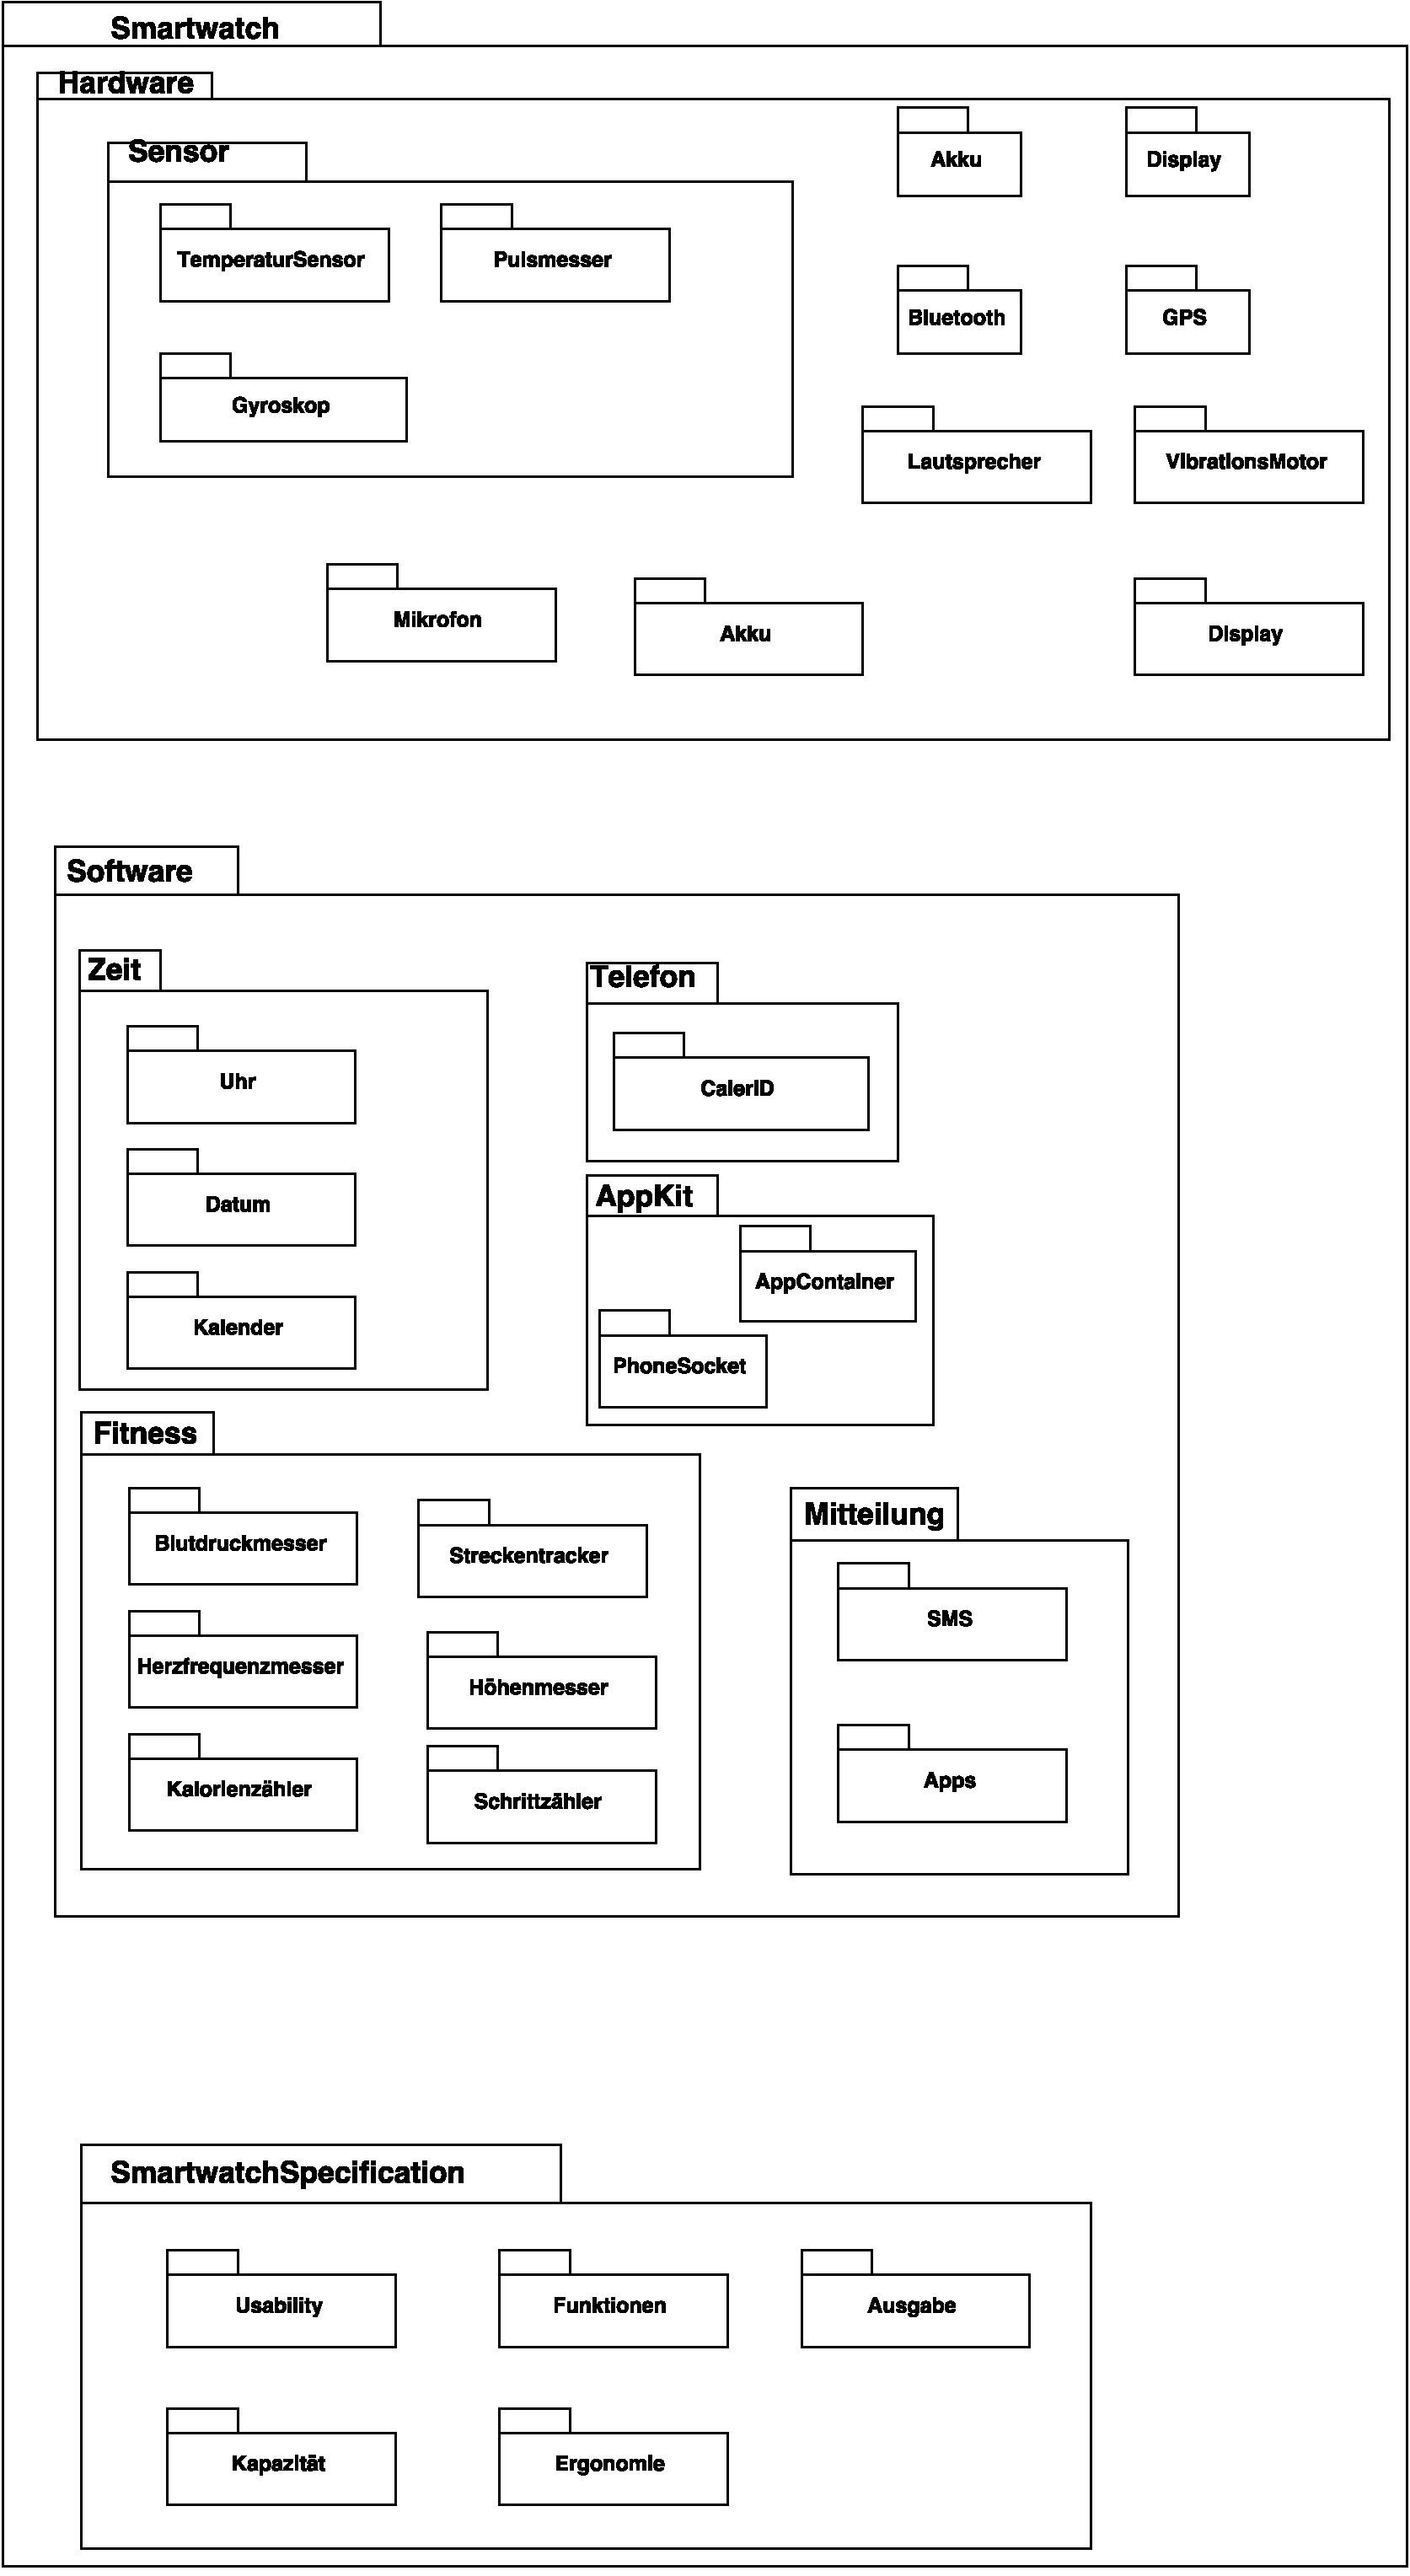
\includegraphics[width=8cm]{img/PackagePhase2}
\caption{Packetdiagramm}\label{fig:package}
\end{figure}

\section{Class Diagram}

\section{Block Definition Diagram}

\section{Timing Diagram}

\section{Parametric Diagram}
Im folgenden wird die Anforderung an die Akkulaufzeit ausführlich als Parametric Diagram dargestellt und erläutert.
Da der Verbrauch des Smartwatches von großem Interesse ist, wird der Verbrauch 
mit Analytische Batteriemodelle modelliert.
Außerdem ist in der Anforderung des Smartwatches festgelegt, das die Akkulaufzeit bei normaler Benutzung mindestens 24 Stunden halten muss. %% ref???
Der Verbrauch eines Systems ist die Summe der Verbrauchswerte einzelner Subkomponenten, wie z.B die Sensoren und Benutzersoftware. Die Subkomponenten dienen als Input für die Laufzeitmodellierung des Smartwatches.
Die Constraint Blöcke dienen der graphischen Repräsentation von Bedingungen für die Ladezeit, die für das Smartwatch verwendet werden sollen. 
Analytische Batteriemodelle sind die erste Klasse der Batteriemodelle, welche
hier näher untersucht werden.
Diese beschreiben mathematisch durch eine oder mehrere analytische Gleichungen den Verbrauch einer Batterie zu modellieren.
Eines der ersten und einfachsten analytischen Batteriemodelle ist die Formel
von Peukert, welche die Entladezeit oder auch tatsächlich nutzbare Kapazität
einer Batterie unter einer konstanten Last berechnen kann.\\ %%%%referenz 
Die Formel von Peukert ist wie folgt:
\[
T= \frac{C}{I^{n}}
\]
Die Kapazität \textit{C} ist in Ampere h gegeben.
\textit{I} steht fur den Strom (in Ampere). Der Parameter \textit{n} steht fur die 
Peukert-Zahl von der verwendeten Batterie.\\
Weiterhin gibt es stochastische Batteriemodelle, dass das Entladeverhalten einer Batterie
über einen stochastischen Prozess modeliert.
Das Modell von Panigrahi ist ein stochastisches Modell.
Im Modell wird zwischen der theoretischen Kapazität \textit{T} und der tatsächlich verfugbaren
Kapazität \textit{N} der Batteriezelle unterschieden.
Die Formel ist in der Constraint-Block abgebildet und in der Literatur näher beschrieben.
In der Abbildung \ref{blockBattery} ist ein Block Definition Diagram angefertigt, welche die einzelnen Constraint Blöcke beinhaltet und ihren inneren Aufbau darstellt.

\begin{figure}[H]
\centering\
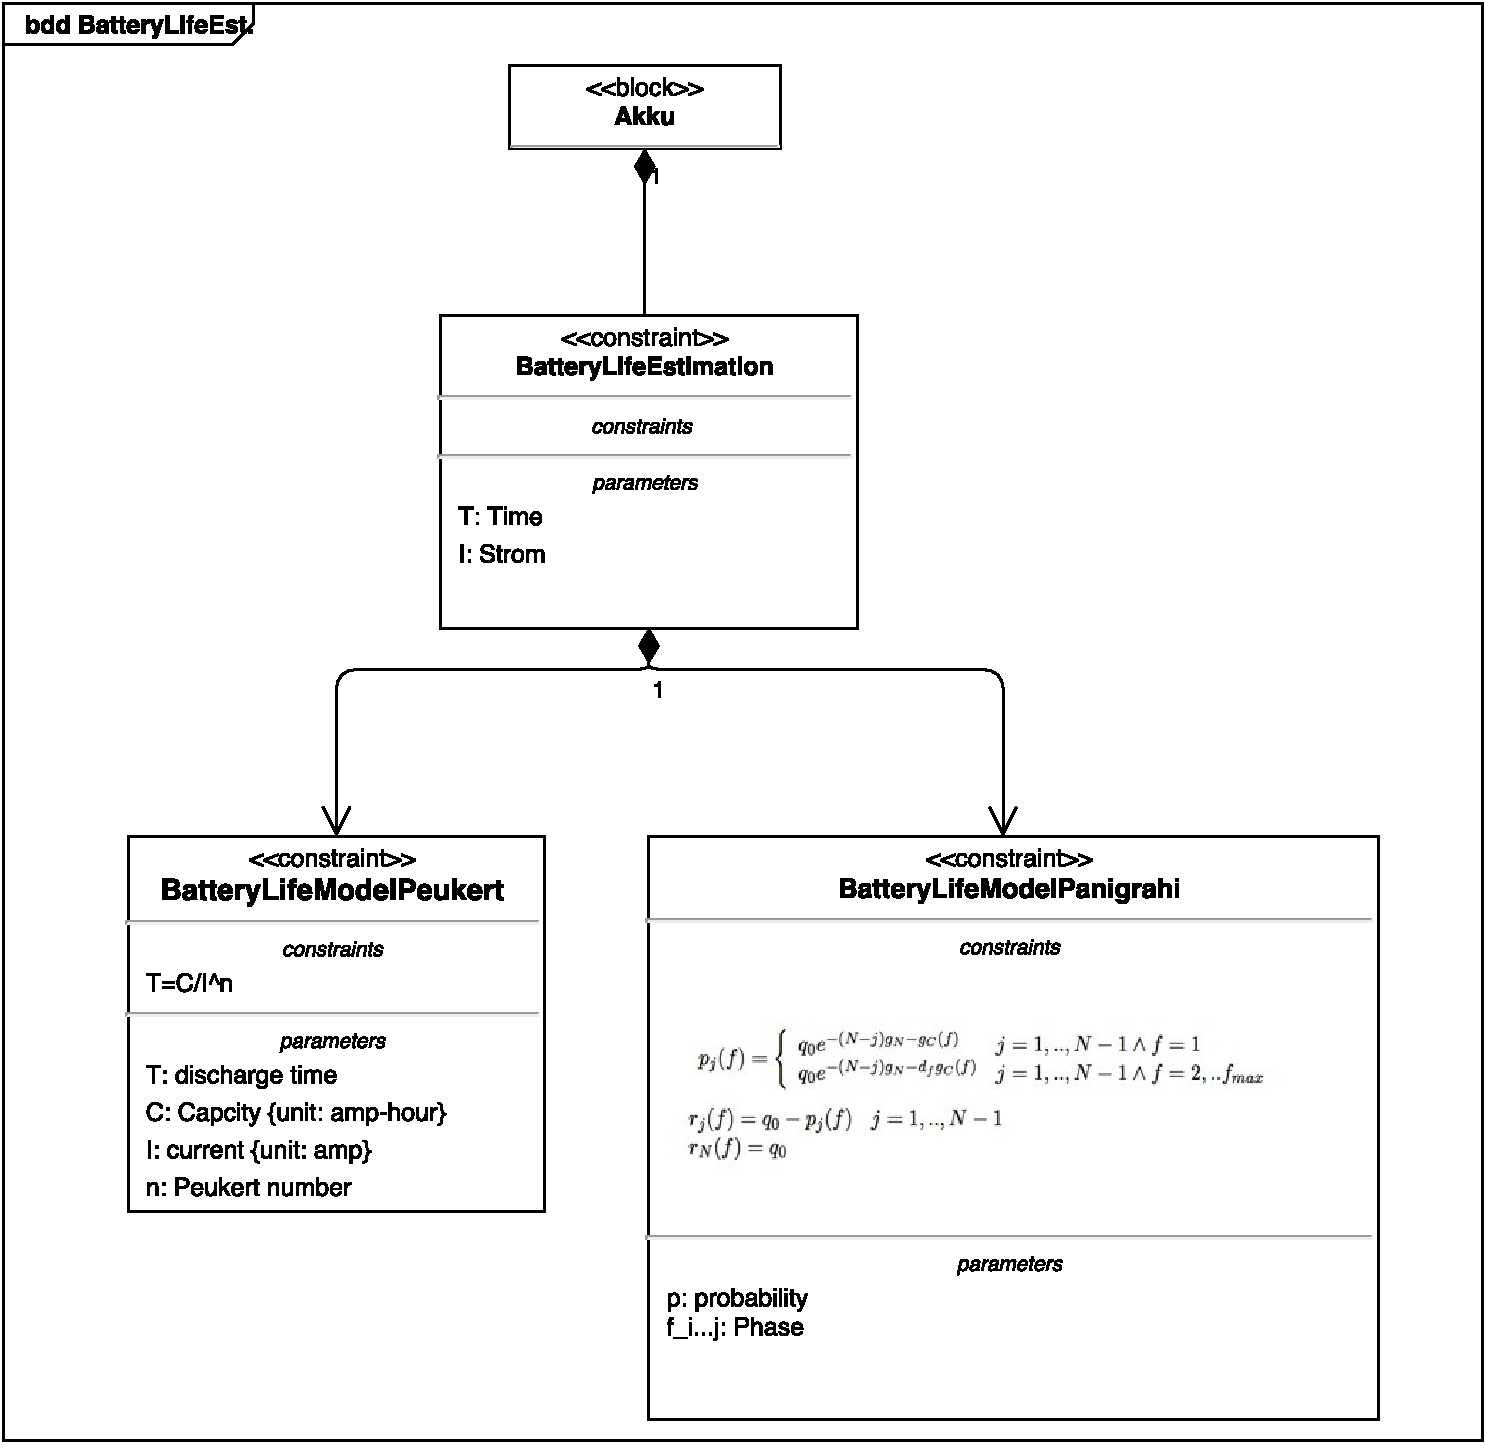
\includegraphics[width=10cm]{img/batterybdd}
\caption{Block Definition Diagram mit den einzelnen Constraint Blöcken}\label{fig:blockBattery}
\end{figure}

Die Verbindungen der einzelnen Systemeigenschaften mit den Constraint-Parameter ist in 
Abbildung \ref{parBattery} dargestellt.
In diesem Diagramm kann man die Beziehungen zwischen den Parametern der einzelnen Constraints und den Systemeigenschaften, hier sind es die Sensoren sehen.

\begin{figure}[H]
\centering\
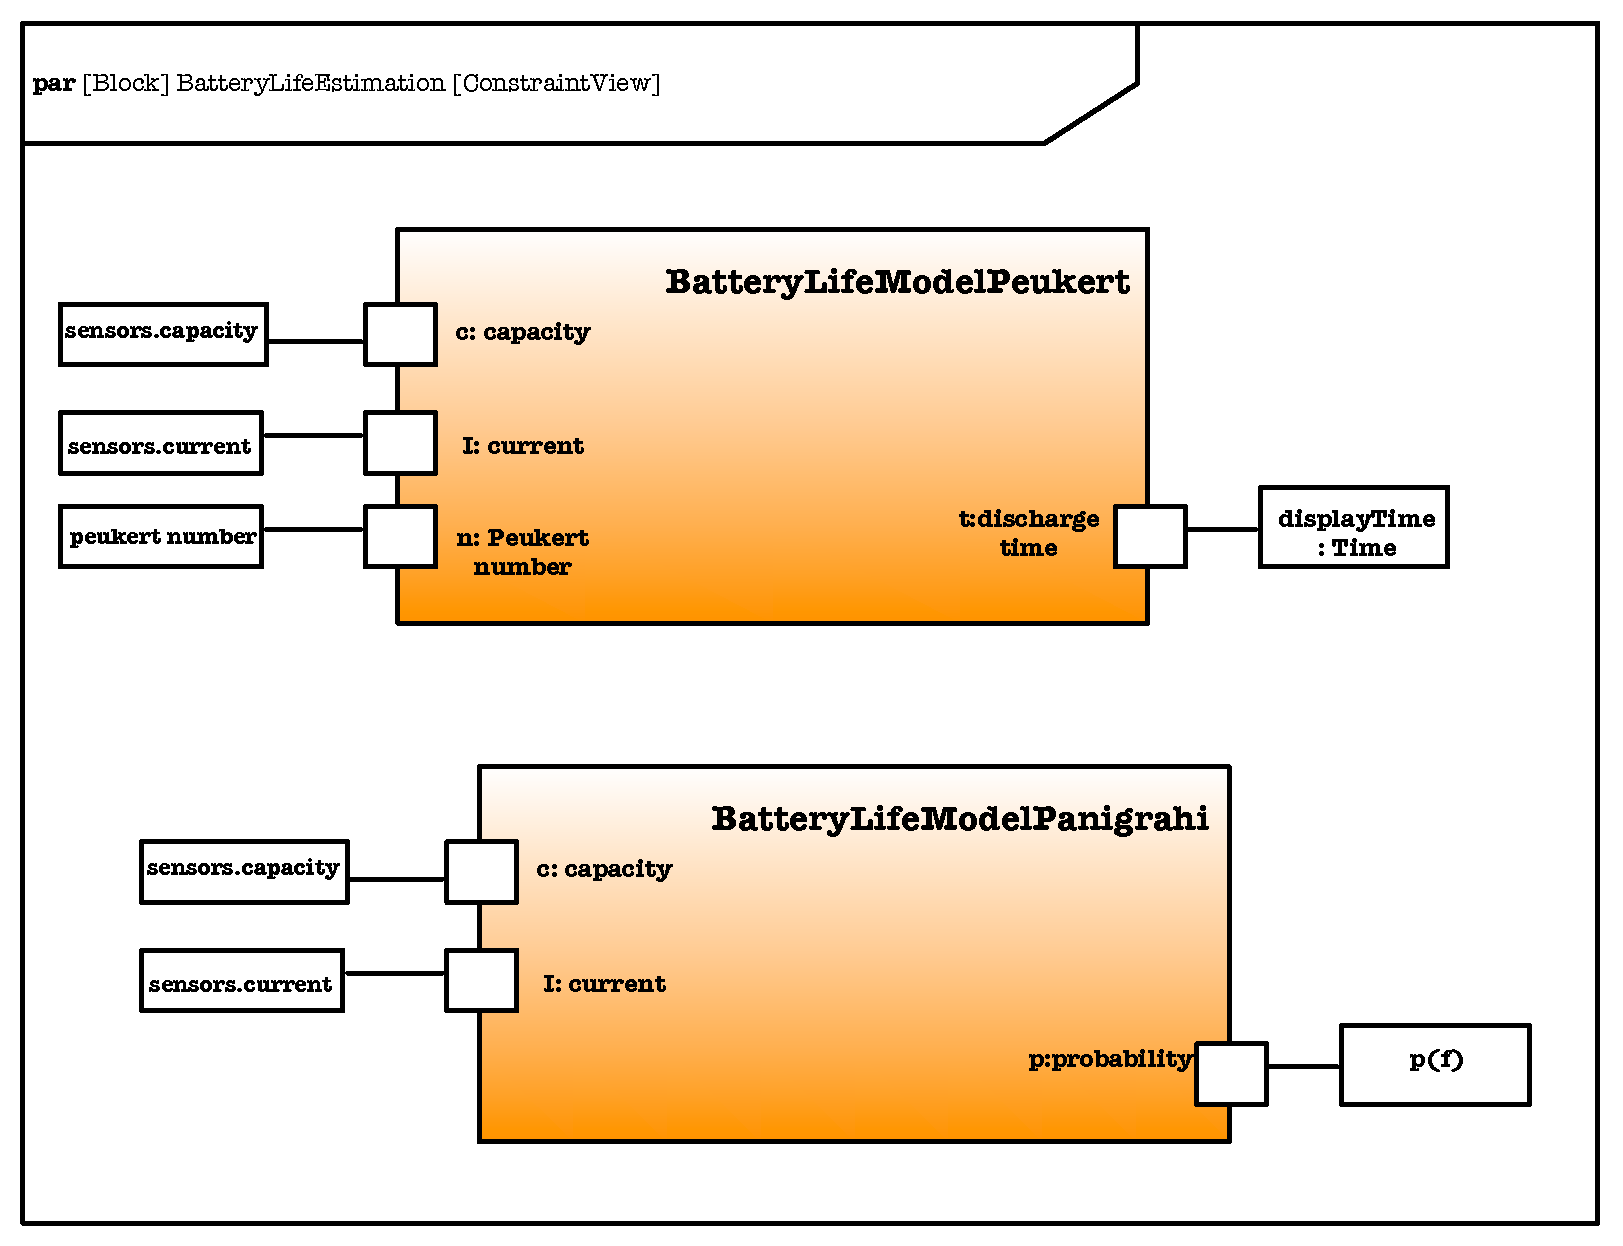
\includegraphics[width=10cm]{img/batteryParametric}
\caption{Parametric Diagram für die Conditions Akkulaufzeit}\label{fig:parBattery}
\end{figure}


\section{Activity Diagram}

\section{Sequence Diagram}

